\formdesc{Mode Commun et Différentiel  : }

\begin{enumerate}
    \item Commun : par rapport à la GND
    \item Différentiel : entre deux potentiels 
\end{enumerate}

\formtitle{Schéma bloc}


\vspace{5mm}

\begin{center}
    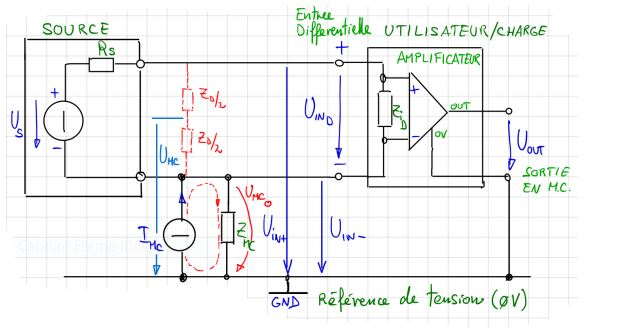
\includegraphics[width = 0.54\textwidth]{img/Schéma.JPG}
\end{center}

Tension mode commun : 
{\hfill$ U_{MC}  = \cfrac{(U_{in+})+(U_{in-})}{2}$ \hfill}

{\hfill$ U_{MC_0}  = I_{MC} \cdot Z_{MC}$ \hfill}

Tension différentielle : 

{\hfill$ U_{D}  = (U_{in+}).(U_{in-})$ \hfill}

\formtitle{Commun Mode Rejection Ratio : CMRR }

Cette grandeur donne l’atténuation d’un signal en entrée en MC sur la sortie :

{\hfill$ CMRR = 20log_{10}\cfrac{U_{in,MC}(f)}{U_{out}(f)}$ \hfill}

\hformbar

